%Chapter 6 will look at the results from the experiments and how the performance of the new software defined radiometer measured up.

\chapter{RESULTS AND ANALYSIS}\label{ch:results}

\section{Introduction}

%Move this section once the stability section is established
To verify stability of the radiometer, we look to see how much change the radiometer records over a relatively long period of time.  To test this a matched load was submerged in a liquid nitrogen bath for an extended period of time, in this case for fifteen minutes.  The readings were then looked at to study the trend of the data.  The data is graphed in figure \ref{Stability}.

\begin{figure}[h!tb] \centering
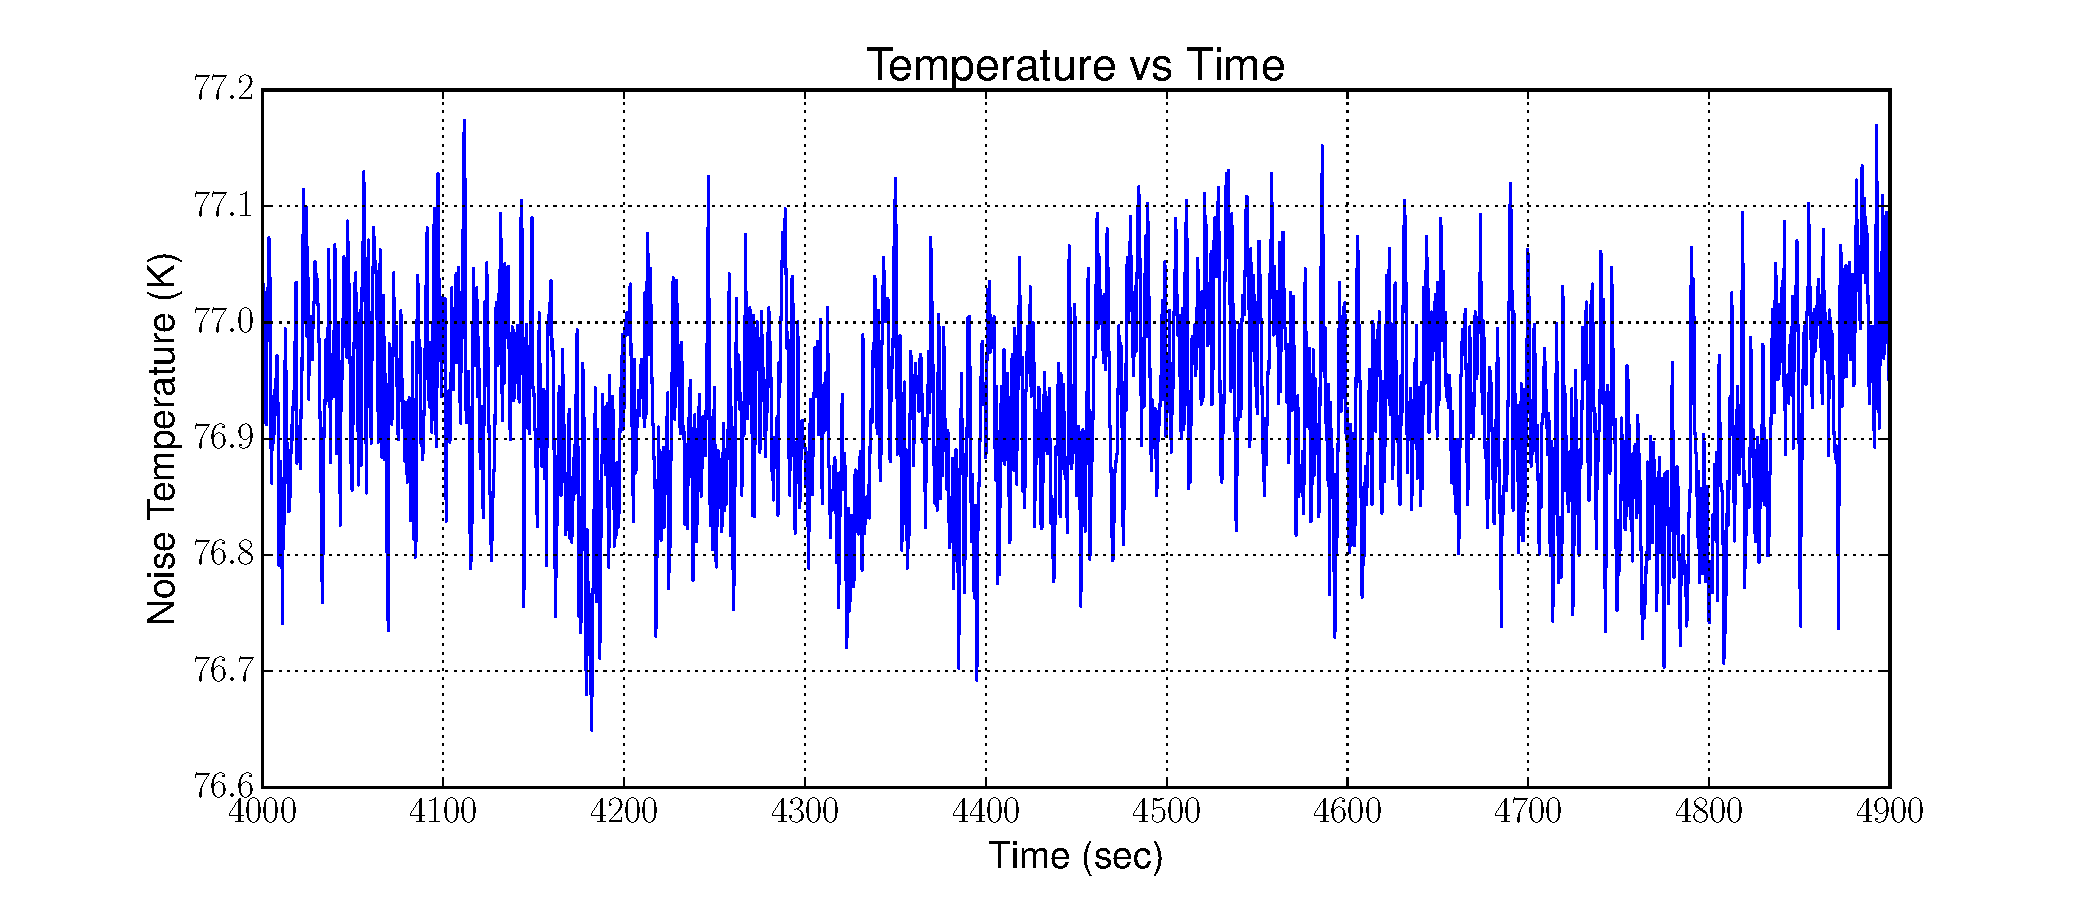
\includegraphics[width=\textwidth]{Experiments/Exp2/sdr_calibrated_zoom.pdf}
\isucaption{Graph of the calibrated total power over a period of fifteen minutes.}
\label{Stability}
\end{figure}

\begin{figure}[h!tb] \centering
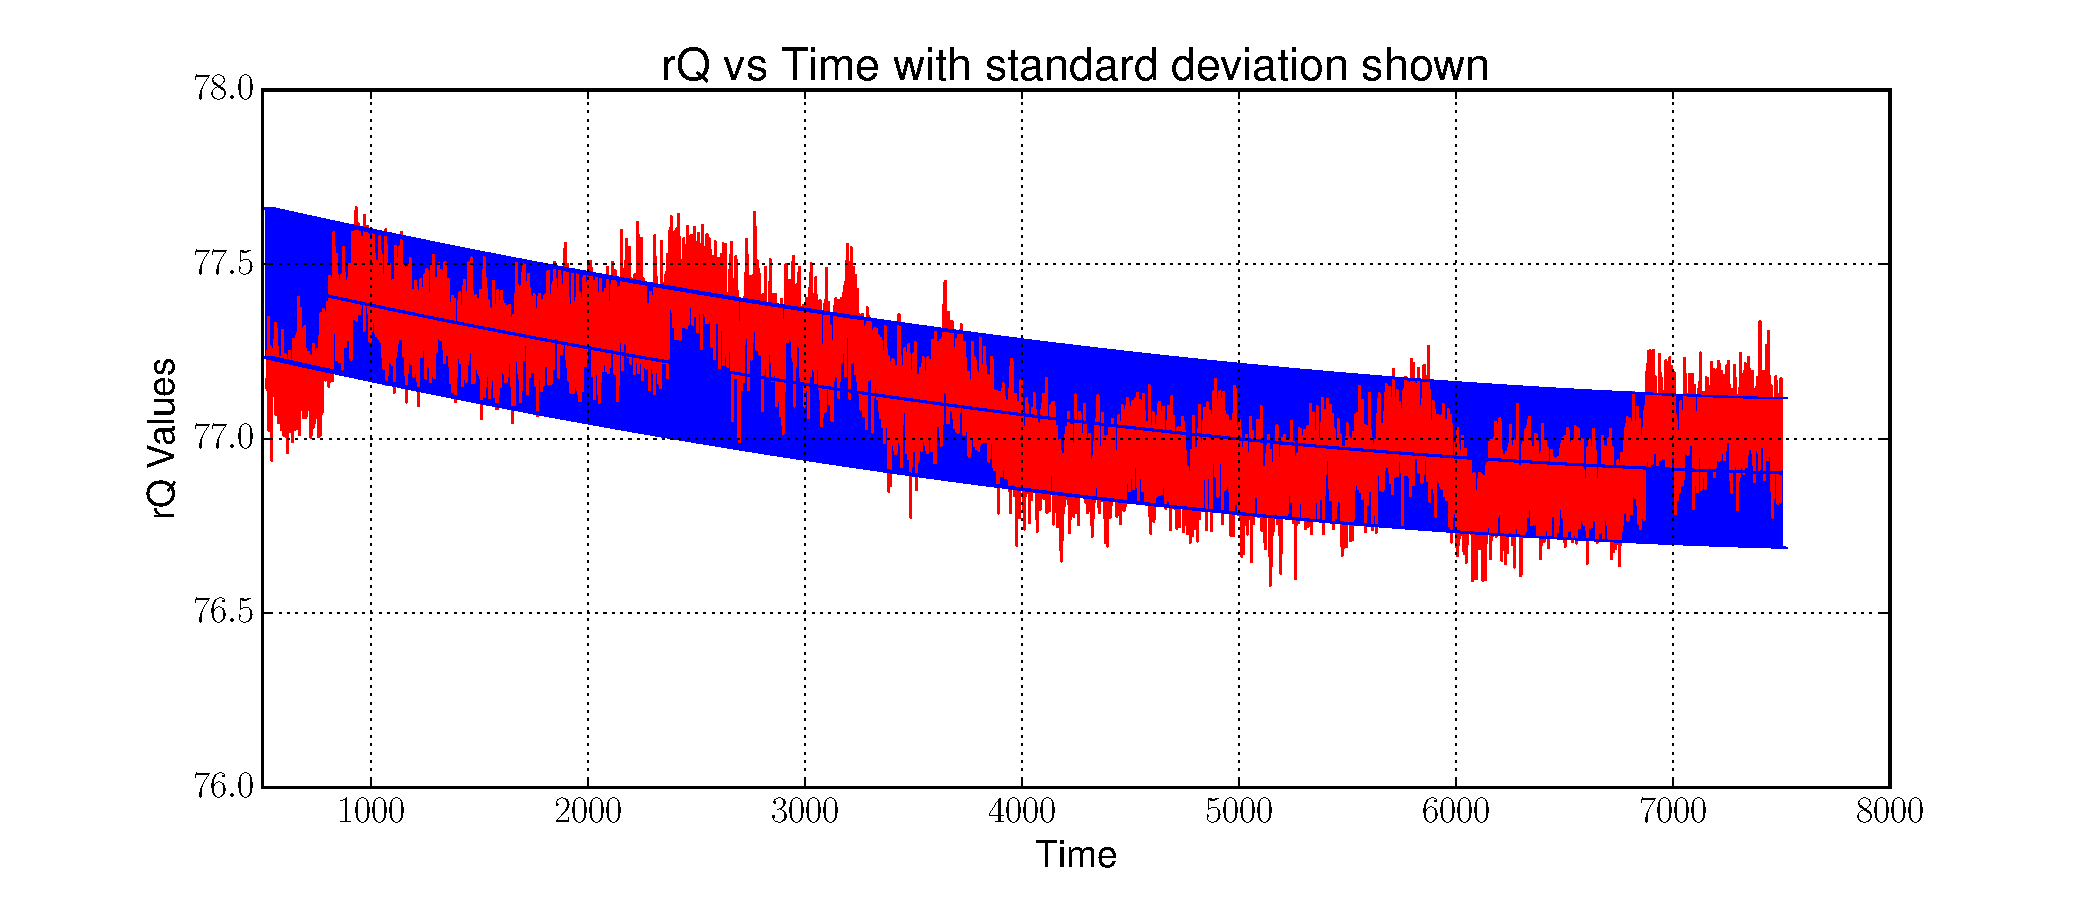
\includegraphics[width=\textwidth]{Experiments/Exp2/calib_vstime_stddev.pdf}
\isucaption{Graph of the calibrated total power with the standard deviation plotted.}
\label{Stability_calib}
\end{figure}

As it can be seen in figure \ref{Stability}, the amount of change over a period of one hour is quite small.  The standard deviation for this sample is 0.09 kelvin.  The $NE\Delta T$ calculated using 10 MHz for the bandwidth, an integration time of 2 seconds and with our sample at 77 Kelvin is calculated to be 0.10 Kelvin with a system temperature of 350 Kelvin.  Therefore, our system is behaving as we expect it to for this stability test.

Figure \ref{Stability_calib} shows a graph of the total readings but with the standard deviation now plotted.  This shows that the system is stable and is operating as expected within our expected $NE\Delta T$.

%---------------------------------------------------------------


Once the experimental data was obtained the next step is to analyze the data and format the data so that it is easy to read and comprehend.  The total power readings and the raw I/Q data generated from GNURadio is stored as a binary file stored in little-endian format.  Total power data is stored as a float values and I/Q data is stored as complex values.  Data from the square-law detector is stored as a comma delimited ASCII file.

Matlab is one tool we can use to process the information that is stored by GNURadio.  Appendix A contains the Matlab source that will read the total power file generated by GNURadio.  It then calculates information such as the NE$\Delta$T and the calibration points based on the user input.  We can also use Matalb to graph this information as well.

While Matlab is one tool, other tools can be used.  Python for example is also capable of reading in these files and when paired with NumPy and SciPy can be used to perform analysis on the data as well [\cite{Uengtrakul}].  In addition, the open source mathematical program Octave should also be able to read and work with these files.  For this thesis both Matlab and Python was used to provide analysis on the data.  

Most of the graphs generated in this thesis was generated using iPython notebooks.  IPython notebooks uses Python but allows it to be executed in a web browser either locally or on a server.  Using iPython notebooks however also allows us to add additional information using Markdown and basic HTML.  This allowed the author to paint a complete picture of the experimental results illustrating pictures of the setup and the code and steps used to analyze the data.  You can find these notebooks on the author's Github site and can use NBViewer to view them.  An example link is \href{http://nbviewer.ipython.org/github/matgyver/Radiometer-SDR-Thesis/blob/master/Experiments/Exp1/radiometer_experiment_1.ipynb}.

{\begin{figure}[h!tb] 
\centering
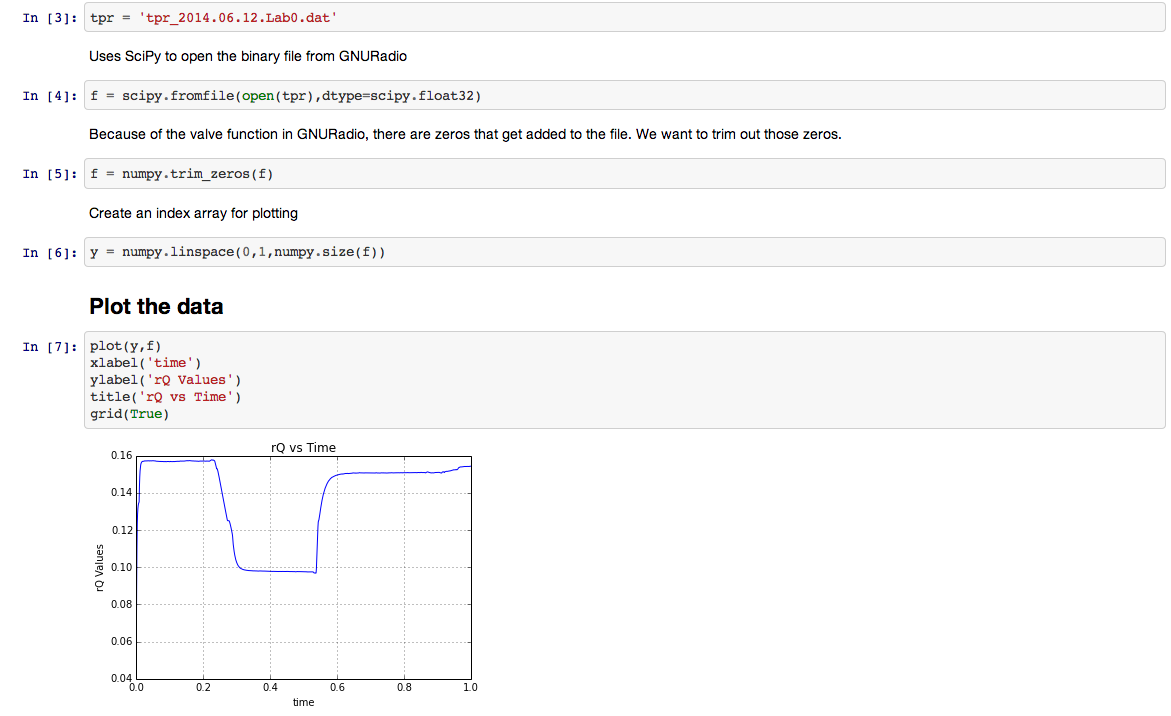
\includegraphics[width=17cm]{Images/python_gnuradio.png}
\isucaption{A screenshot showing the iPython notebook code and related graphs generated for parsing GNURadio data}
\label{matlab_display}
\end{figure}


\section{Benefits to Software Defined Radio Radiometer}
A study was conducted on what benefits a software defined radio radiometer would have over a more traditional radiometer.  This was focused on looking at three main areas; cost, weight and size, and the value a SDR radiometer can add over traditional radiometers.

\subsection{Cost Benefits}
Software defined radios have become more commonplace in recent years and this has generated a number of Commercial Off The Shelf (COTS) solutions.  A COTS solution is often a lower cost solution due to the mass manufacturing that takes place.  This has driven the cost of many SDRs to under one thousand dollars while still having excellent performance characteristics.  The N200 SDR purchased for this research cost fifteen hundred dollars and the daughter-board cost one hundred and fifty dollars approximately.  Other software defined radios however have come out on the market since then.  Ettus for example has some that are below one thousand dollars and the author has also obtained the HackRF One SDR that now sells for three hundred dollars.  The main difference with the different software defined radios on the market is with both the resolution, or how many bits the ADC is, and the bandwidth they are able to handle.

\begin{table}[h!tb] \centering
\isucaption{Cost Analysis}
\label{cost_table}
% Use: \begin{tabular{|lcc|} to put table in a box
\begin{tabular}{lcc} \hline
\textbf{Device} & \textbf{Quantity} & \textbf{Cost} \\ \hline
\textbf{SDR Solution}& & \\ \hline
N200 SDR & 1 & \$1515 \\
LNA at \$60 ea. & 3 & \$180 \\
DBSRX2 Daughter-board & 1 & \$152 \\
GNURadio & 1 & \$0 \\ \hline
Total & & \$1847 \\ \hline
\textbf{ISU Radiometer} \\ \hline
LNA, FPGA, ADC, Microcontroller and power supplies & 1 & \$10,000\tablefootnote{Purchase price in 2005} \\ \hline
\textbf{Commercial Off the Shelf Unit}\\ \hline
Spectracyber 1420 MHz Hydrogen Line Spectrometer & 1 & \$2,650 \\ \hline

\end{tabular}
\end{table}

As see in table \ref{cost_table}, even the higher cost Ettus research equipment is a lower cost option than the custom built ISU radiometer purchased from University of Michigan and even a comparable off the shelf radiometer.  It should be noted that the radiometer from the University of Michigan is also a dual polarization radiometer so there are two RF front ends and two ADCs that feed into a FPGA board.  It would be quite easy to add dual polarization to the Ettus N200 SDR as it does support two daughter-boards.  This would increase the cost to \$2,179 for the additional LNAs and daughter-board.

The largest cost benefit is that key components that you find in a radiometer, the filters and square-law detector can now be all done in software instead of needed additional equipment.  The system is also much more frequency agile, which means it can work on a broader range of frequencies than most traditional radiometers with very little change in hardware and in some cases may require no change in hardware.  Some of this does depend on the SDR hardware however.  The Ettus N200 for example uses daughter-boards to provide the RF interface.  While these boards provide a high quality in the RF signal, it does come at a cost and are usually designed for certain bands of frequencies.  Other low cost SDRs however are also very wide range in the frequencies they will work in.  The HackRF for example works from 10 MHz to 6 GHz, but does so at the cost of lower resolution, less gain in its front end and a lower bandwidth that it can handle.

\subsection{Weight and component size benefits}

A typical radiometer has many components that are involved in the design of the radiometer.  This includes filters, LNAs and the power detection or square-law detector used.  These components add both weight, size and costs to the radiometer.  A software defined radio however digitizes the signal and we are able to replace the filters and square-law detector with their software equivalent.  While a software defined radio does add both the ADC and usually a FPGA to do the processing on the signal, advances in semiconductor technology has continued to shrink these components.  These components are also lighter than the filters often used in radiometers.

\begin{table}[h!tb] \centering
\isucaption{Weight Analysis}
\label{weight_table}
% Use: \begin{tabular{|lcc|} to put table in a box
\begin{tabular}{lc} \hline
\textbf{Device} & \textbf{Mass} \\ \hline
\textbf{SDR Solution} & \\ \hline
N200 SDR & 1.2 kg \\
LNA at .03 kg ea & .09 kg \\
DBSRX2 Daughter-board & .1 kg \\ \hline
Total & 1.39 kg \\ \hline
\textbf{ISU Radiometer} \\ \hline
LNA, FPGA, ADC, Microcontroller and power supplies & 22.7 kg \\ \hline
\textbf{Commercial Off the Shelf Unit}\\ \hline
Spectracyber 1420 MHz Hydrogen Line Spectrometer & 6 kg\tablefootnote{Estimated, no data available} \\ \hline

\end{tabular}
\end{table}

Size is another benefit as since semiconductor technology has continued to shrink components.  Again, since items like the filters and square-law detector are removed and done in software this helps to reduce the overall size.  

\subsection{Value added benefits}

A software defined radio radiometer adds additional value for two reasons.  One, it is able to work with both frequency and magnitude where most radiometers do not.  This allows for additional analysis on the signal and can help identify issues such as an interfering signal that was demonstrated in this thesis.  

Second, we are able to have an agile system that is able to adapt to changing conditions with very little or no change to hardware.  Different types of radiometers can be implemented such as a Dicke radiometer, dual polarization radiometer or a radiometer that can perform Stokes parameters.  In addition, since we have both frequency and power information we can create a system that is able to adapt to changing conditions such as dealing with an interfering signal.  

\section{Disadvantages of a SDR Radiometer}
Although we have outlined a number of advantages of using a COTS SDR Radiometer and how a SDR can add additional value to the radiometer system, there are some disadvantages to a SDR Radiometer.

\subsection{Power Consumption}
One of the largest drawbacks to a SDR radiometer can be in the power consumption of the SDR.  With the move to perform functions such as power detection and filtering we now require additional computational power to perform these tasks.  With those computational cycles additional power is now required.  The use of FPGAs and SoC however can help to minimize these power concerns as they are more efficient than using a full scale x86 based processor and on board computer system.  

Power and CPU requirements also increase as we add additional functionality such as filtering an offending signal.  While these additions may not require additional hardware, it can require additional processor or computational requirements.  This will cause additional strain on the processor and also in the memory requirements for the SDR as well.

\subsection{Bandwidth constraints}
While SDR technology has advanced, bandwidth is still a constraint that affects SDRs and in turn a SDR Radiometer.  Bandwidth plays a critical role in the radiometer's sensitivity as explained in this thesis, therefore the fact that many SDRs are limited in bandwidth does create a disadvantage.  In many cases this bottleneck takes place in both the transport and processing of large bandwidth systems.  This also relates to the power consumption disadvantage since larger bandwidth also means requiring additional computational cycles as well.  

In contrast, a square-law detector usually has a very large bandwidth, as much as one gigahertz, and is why we usually need to filter to the frequency band of interest.  

\section{Results Summary}

%----------------------------------------------------------
% End of Chapter 6.  Anything below this is extra information